

% !TEX root = ../popl-paper.tex

In synchronous communication (also known as rendezvous communication), send and receive events are  viewed as a single entity, i.e., a receive event  happens simultaneously with its corresponding send. The  idea behind (fully) asynchronous communication, instead, is to decouple send and receive events, so that a receive event can happen indefinitely after its corresponding send. Depending on some additional constraints on those events, we can obtain new communication models that sit somewhere between synchronous and fully asynchronous communication.
In this paper we try to clarify and classify some communication models.  We consider only point-to-point communication, that is, messages that have exactly one sender and one receiver.  We follow the classification introduced in \cite{DBLP:journals/fac/ChevrouHQ16} but we generalize the models to  consider unmatched messages (i.e., messages that have been sent, but not yet read). Another major difference is that in \cite{DBLP:journals/fac/ChevrouHQ16} only single executions are considered, whereas we are interested in classes of executions represented by \emph{Message Sequence Charts} (MSCs in the following) \cite{messagesequencecharts}.
MSCs are a graphical representation of the  computations of distributed systems.  Roughly speaking, a distributed system is composed by a set of sequential processes that can exchange messages. Each process exhibits a sequence of \emph{events}, which in our case will be either \emph{send} or \emph{receive} events. A send event $s$ and a receive event $r$ are said to be \emph{matching} if the message sent by $s$ is the same  that is received by $r$. A distributed computation is the concurrent execution of each process. In an MSC, such as the one in Fig.~\ref{fig:msc_ex}, each vertical line is called a \emph{process line} and it represents the order in which events are executed by a single process, with time running from top to bottom; arrows are used to represent messages and they connect a send event with its corresponding matching receive. 
Given a message $m_i$, we will use $!i$ and $?i$ to denote the corresponding two matching send and receive events. A single process line defines a total order over the events executed by that process, i.e., an event $e$ happens before another event $e'$ if $e$ is higher in the process line; in Fig.~\ref{fig:msc_ex}, if we look at process $q$ we see that $?1$ happens before $?2$. However, in general MSCs only specify a partial order over events. Consider the events $!1$ and $!2$ in Fig.~\ref{fig:msc_ex}, which are executed by two different processes; these two events are said to be \emph{concurrent}, in the sense that this MSC does not tell us which one is executed first. 
Nonetheless, even though events on different processes can be concurrent, this is not always the case. For instance send events must always happen before their corresponding matching receive. Graphically, this \emph{happens before} relation between events on different processes is represented by a path that follows the direction of the arrows and runs from top to bottom. This will be referred to as a \emph{causal path}, because it estabilishes a causal relation between events (cfr. the red annotations in  Fig.~\ref{fig:msc_ex}). 
%Consider events $!1$ and $?2$ of the MSC shown in Fig.~\ref{fig:msc_ex}. Even though they are executed by different processes, $?2$ must happen before $!1$ because $?2$ must be executed after $!2$, which happens before $?1$, which in turn happens before $!1$. 
%The fact that $!1$ is higher on his own process line compared to $!2$ does not meaning anything with respect to the order in which they are executed. 
Since an MSC defines a partial order over the events of a distributed system, it can always be extended to a total order, which will be referred to as a \emph{linearization}. 
%Given an MSC, it can have multiple linearizations. For the MSC in Fig.~\ref{fig:msc_ex}, both $!1\;?1\;!2\;?2$ and $!2\;!1\;?1\;?2$ are valid linearizations, i.e. a total order over the events which is compatible with the partial order defined by the MSC. 
Intuitively, a linearization represents the order in which events are executed by the distributed system according to \emph{absolute time}, i.e. as they are seen by an external viewer that has a global view of all the processes. 

\begin{figure}[t]
	\begin{center}
		\begin{tikzpicture}
			\newproc{0}{p}{-2.5};
			\newproc{1}{q}{-2.5};
			\newproc{2}{r}{-2.5};
		
			\newmsgm{0}{1}{-0.5}{-0.5}{1}{0.5}{black};
			\newmsgm{2}{1}{-1.2}{-1.2}{2}{0.5}{black};
			\newmsgm{1}{0}{-1.9}{-1.9}{3}{0.5}{black};

			\newflechehorinverse{Purple}{-1.2}{2}{1};
			\newflechevert{Purple}{1}{-1.3}{-2.0};
			\newflechehorinverse{Purple}{-1.9}{1}{0};

			\newevent{black}{0}{-0.5}{!1}{left};
			\newevent{black}{1}{-0.5}{?1}{right};
			\newevent{black}{2}{-1.2}{!2}{right};
			\newevent{black}{1}{-1.2}{?2}{left};
			\newevent{black}{1}{-1.9}{!3}{below right};
			\newevent{black}{0}{-1.9}{?3}{left};

		\end{tikzpicture}
		\caption{An example of MSC. A causal path between $!2$ and $?3$ is highlighted with red arrows.}
		\label{fig:msc_ex}
	\end{center}
\end{figure}

\cinzia{Have a look at \url{https://web.archive.org/web/20060826195305/http://www.comp.nus.edu.sg/~thiagu/public_papers/surveymsc.pdf}}

\cinzia{\url{https://link.springer.com/content/pdf/10.1007/978-0-387-35271-8.pdf} to mention while talking about realizability page 81-96}

Going back to our contribution, the work in \cite{DBLP:journals/fac/ChevrouHQ16} describes the properties that a single linearization must satisfy in order to be realizable by a system that uses a given communication model. On the other hand, we are interested in understanding if a given MSC describes a computation that can be realized by a system that uses some communication model $CM$. In other words, given a MSC we want to know if it has at least one linearization that respects the constraints imposed by $CM$. If that is the case, the MSC represents a behaviour that can be exhibited by a system that uses $CM$ as a communication model. These are two fundamentally dissimilar problems; at the end of this section we provide an example to clarify the difference. In our work, we are going to formally characterize the classes of MSCs which represent valid computations for all of these 7 communication models. We also show how these classes form a well-defined hierarchy, which does not correspond entirely to that found in \cite{DBLP:journals/fac/ChevrouHQ16}.

\cinzia{talk about realizations here?}

\cinzia{say that the two hierarchy differs}
\paragraph{Contributions.}\cinzia{to rewrite here}

We find of particular interest to study the relation between the classes of MSCs for all of these communication models. For instance, the MSC shown in Fig.~\ref{fig:co_ex} is both asynchronous and $\oneone$, in the sense that we are able to find systems using those communication models that can produce the behaviour described by the MSC. Is it always the case than a $\oneone$ MSC is also an asynchronous MSC? What about the other communication models? In Section~\ref{sec:hierarchy} we prove that the classes of MSCs for all these communication models form a very neat hierarchy, which is graphically shown in Fig.~\ref{fig:msc_hierarchy_full}.

% \cinzia{redo fig in tikz}
% \begin{figure}[h]
% 	\centering
% 	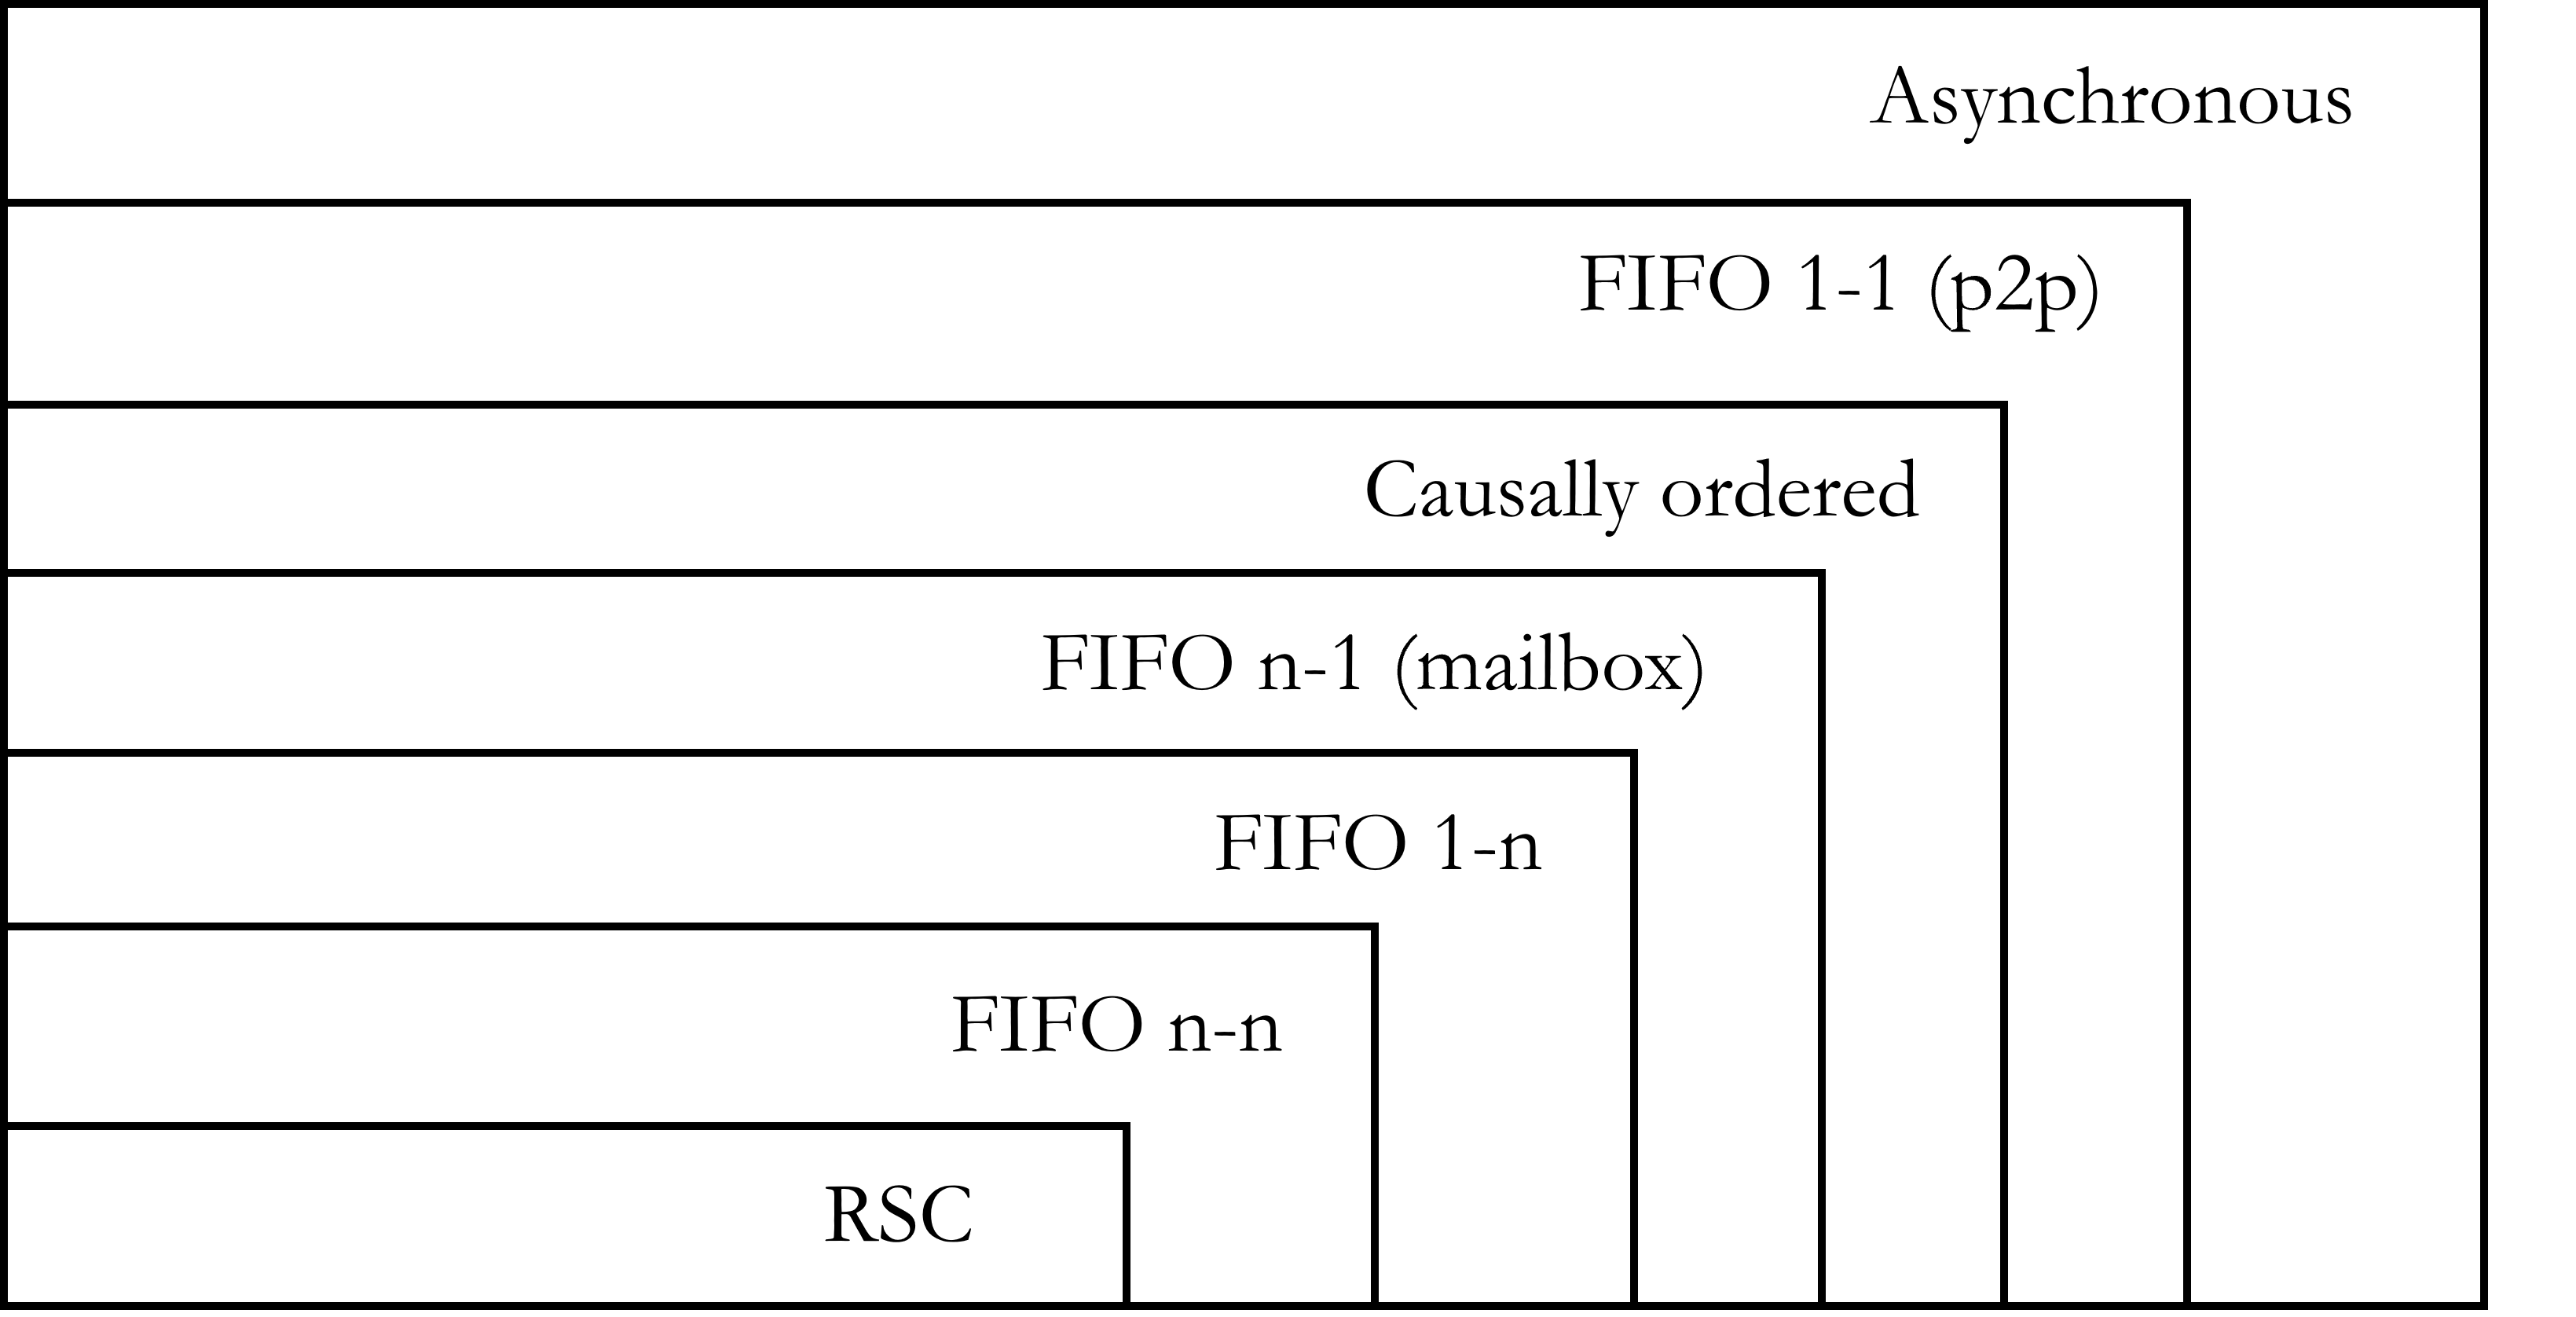
\includegraphics[width=8cm]{msc_hierarchy}
% 	\caption{The hierarchy of MSC classes.}
% 	\label{fig:msc_hierarchy_full}
% \end{figure}

\begin{figure}[h]
	\centering
	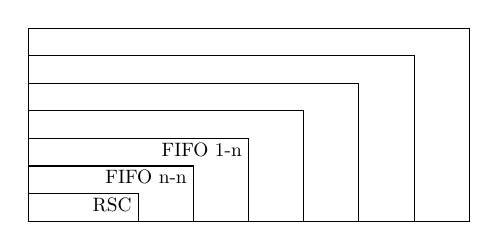
\begin{tikzpicture}[scale=0.7, every node/.style={transform shape}]
		\draw  (0,0) rectangle (2,.5);
		\draw (2,0.3) node[left]{RSC};
		\draw  (0,0) rectangle (3,1);
		\draw (3,0.8) node[left]{FIFO n-n};
		\draw  (0,0) rectangle (4,1.5);
		\draw (4,1.3) node[left]{FIFO 1-n};
		\draw  (0,0) rectangle (5,2);
		\draw (5,1.8) node[left]{\mb};
		\draw  (0,0) rectangle (6,2.5);
		\draw (6,2.3) node[left]{\co};
		\draw  (0,0) rectangle (7,3);
		\draw (7,2.8) node[left]{\pp};
		\draw  (0,0) rectangle (8,3.5);
		\draw (8,3.3) node[left]{\asy};
	\end{tikzpicture}
	\caption{The hierarchy of MSC classes.}
	\label{fig:msc_hierarchy_full}
\end{figure}


\cinzia{add fig. of decidability results}

\paragraph{Outline.} The paper is organized as follows. Section \ref{sec:com_models_overview} details the communication models we consider.  Then, Section \ref{sec:MSO} gives a formal definition of MSC realizing a given communication model and characterizes the classes of MSCs via MSO logic. Finally, Sections \ref{sec:hierarchy} and \ref{sec:checking} show respectively how the different communication models are related and use this information to show some (un)decidability model checking results that follow from the notion of special treewidth.

